% ==================================================================
%  Shared-Control Teleoperation of Unknown Constrained Mechanisms
%  Literature review and proposed Franka--DualSense architecture
%  Compile:  pdflatex main  ->  biber main  ->  pdflatex main  (x2)
%            or simply:  latexmk -pdf main.tex
% ==================================================================
\documentclass[11pt,letterpaper]{article}

% ---------- page layout: 1 inch margins on all sides ---------------
\usepackage[margin=1in]{geometry}

% ---------- fonts and encoding -------------------------------------
\usepackage[T1]{fontenc}
\usepackage[utf8]{inputenc}
\usepackage{lmodern}
\usepackage{microtype}

% ---------- mathematics --------------------------------------------
\usepackage{amsmath,amssymb,bm}

% ---------- tables, figures, algorithms ----------------------------
\usepackage{graphicx}
\usepackage{booktabs}
\usepackage{tabularx}
\usepackage{array}
\usepackage{multirow}
\usepackage[font=small,labelfont=bf]{caption}
\usepackage{subcaption}
\usepackage{algorithm}
\usepackage{algpseudocode}
\usepackage{pdflscape}
\usepackage{afterpage}

% ---------- drawing ------------------------------------------------
\usepackage{xcolor}
\usepackage{tikz}
\usetikzlibrary{positioning,arrows.meta,fit,backgrounds,calc,shapes.misc,angles,quotes}

% ---------- bibliography -------------------------------------------
\usepackage[backend=biber,style=ieee,sorting=none,doi=true,url=false,eprint=true]{biblatex}
\addbibresource{references.bib}

% ---------- links (load late) --------------------------------------
\usepackage[colorlinks=true,linkcolor=blue!50!black,citecolor=blue!50!black,urlcolor=blue!50!black]{hyperref}
\usepackage[capitalise,noabbrev]{cleveref}

% ---------- notation -----------------------------------------------
\newcommand{\vect}[1]{\bm{#1}}
\newcommand{\dhat}{\hat{\vect{d}}}
\newcommand{\Pd}{\mathbf{P}_{\hat d}}
\newcommand{\I}{\mathbf{I}}
\newcommand{\vuser}{\vect{u}}
\newcommand{\vcmd}{\vect{v}_{c}}
\newcommand{\Fext}{\vect{F}}
\newcommand{\Fperp}{\vect{F}_{\perp}}
\newcommand{\Fpar}{F_{\parallel}}
\DeclareMathOperator{\sat}{sat}

% ---------- colours used in the diagrams ---------------------------
\definecolor{opcol}{RGB}{226,236,248}
\definecolor{sccol}{RGB}{232,245,233}
\definecolor{robcol}{RGB}{252,240,226}
\definecolor{hapcol}{RGB}{190,40,40}
\definecolor{viscol}{RGB}{90,90,90}
\definecolor{estcol}{RGB}{30,110,60}

\begin{document}

% ---------- title (no author or date block) -------------------------
\begin{center}
  {\LARGE\bfseries Shared-Control Teleoperation of\\[2pt] Unknown Constrained Mechanisms\par}
  \vspace{6pt}
  {\large\bfseries A Literature Review and a Proposed Franka--DualSense Architecture\par}
\end{center}
\vspace{6pt}

% ==================================================================
\begin{abstract}
Opening a drawer or a door is effortless for a person standing in front of it, yet the same motion becomes delicate when it is carried out remotely through a robot arm. Once the gripper holds the handle, arm and mechanism form a closed kinematic chain, and any commanded motion that departs from the single direction the mechanism permits is converted into internal force at the handle. An operator working through a gamepad can neither feel these forces nor know in advance which way the mechanism moves. This paper reviews the literature bearing on that problem and proposes a control architecture for studying it. The review is anchored on Lutscher et al.\ \cite{lutscher2010control}, who estimate the permitted direction of an unknown one-degree-of-freedom mechanism from the measured end-effector motion, and places that work among ten recent studies of articulation estimation, shared control and haptic feedback published between 2021 and 2026. The proposed architecture lets an operator command Cartesian velocity with a Sony DualSense controller while an online estimator follows the local tangent of the mechanism; in the assisted mode the command is projected onto this tangent in the manner of a guidance virtual fixture. Off-axis force is conveyed through vibration and opening resistance through the controller's adaptive trigger, so that direct and assisted teleoperation can be compared under identical feedback.
\end{abstract}

% ==================================================================
\section{Introduction}
\label{sec:intro}

Doors, drawers, cabinet lids and appliance doors are among the objects a service or assistive robot is most often expected to operate. Each is a one-degree-of-freedom mechanism: a drawer slides along a prismatic joint and a door swings about a revolute hinge. When the robot has grasped the handle firmly, arm, gripper and mechanism form a closed kinematic loop, and the end-effector is no longer free to move in arbitrary directions. Only motion along the mechanism's path is admissible. Displacement commanded in any other direction is resisted by the cabinet or the door frame, and on a stiff, position-controlled arm that resistance appears as contact forces large enough to damage the hardware, pull the handle out of the gripper or trip the robot's safety limits.

Autonomous approaches to this problem differ mainly in how much they assume about the mechanism. Model-based methods first locate the hinge or slide axis, usually from vision, and degrade when that estimate is wrong. A second family dispenses with the model and lets the mechanism reveal itself through contact. The robot is made compliant, pushed gently in a plausible direction, and the direction in which the end-effector actually moves is taken as the direction the mechanism allows \cite{niemeyer1997simple,lutscher2010control,karayiannidis2013modelfree}. The present work belongs to this second family.

What distinguishes it from the autonomous literature is the presence of a human operator, who drives a Franka Panda arm with a DualSense game controller while the arm holds the handle of a drawer or door whose motion is not known in advance. Teleoperation is attractive in this setting because the operator supplies what autonomous systems still find difficult, namely deciding what to open and judging from the scene roughly how it opens. Large-scale field studies of autonomous opening support this view, identifying perception rather than low-level control as the dominant source of failure \cite{gupta2025opening}. The operator, however, introduces difficulties of a different kind. A thumbstick gives only coarse directional input, the forces at the handle cannot be felt, and the relation between stick deflection and end-effector velocity in a rotated drawer frame is far from intuitive. Operators therefore tend to push partly into the side of a drawer, or along the chord of a door's arc, and the robot ends up working against the mechanism.

The control problem can thus be stated as \emph{compliant manipulation under an unknown kinematic constraint, avoiding forces perpendicular to the permitted motion}. The approach developed here combines two ideas from different parts of the literature. The first is the online direction estimator of Lutscher et al.\ \cite{lutscher2010control}, which tracks the instantaneous direction of permissible motion from the measured end-effector velocity. The second is the guidance virtual fixture \cite{rosenberg1993virtual,marayong2003spatial,abbott2003architectures}, which filters an operator's command by projecting it onto a preferred subspace. Together they yield an assistance law of the form $\vcmd = \hat{\vect{d}}\hat{\vect{d}}^{\top}\vuser$, where $\vuser$ is the operator's velocity command and $\hat{\vect{d}}$ the estimated tangent of the mechanism. On the operator's side the DualSense closes the loop: its rumble motors signal that the operator is pushing against the constraint, and its adaptive trigger stiffens when the mechanism itself is hard to open.

The architecture is designed around a single comparison. Under \emph{direct} control the robot follows the operator's Cartesian command unchanged, while under \emph{assisted} control the command is projected onto the estimated permitted motion. Both modes provide the same haptic feedback, so that differences in opening time, off-axis force, handle loss and achieved opening distance can be attributed to the assistance itself. A prismatic drawer with a randomised axis is the primary task, and the hinged door and fully unfamiliar mechanism are treated as extensions.

\Cref{sec:litreview} reviews the primary paper, the classical work it builds on, and ten recent studies. \Cref{sec:architecture} presents the proposed architecture as an annotated block diagram and derives its estimation, assistance and haptic laws. \Cref{sec:conclusion} summarises the contribution.

% ==================================================================
\section{Literature Review}
\label{sec:litreview}

The review begins with the primary paper, which defines the technical core of this work, and briefly recalls the older results on compliant mechanism operation and virtual fixtures on which it rests. It then turns to recent research in three areas: estimating and following kinematic constraints, sharing control between operator and robot, and conveying contact information through the operator interface. A comparative summary closes the section and identifies the gap the proposed architecture addresses.

% ------------------------------------------------------------------
\subsection{Primary Paper: Operating Unknown Constrained Mechanisms}
\label{sec:primary}

Lutscher, Lawitzky, Cheng and Hirche \cite{lutscher2010control} study a manipulator that has grasped the handle of a mechanism whose single degree of freedom is unknown, using everyday objects such as drawers, cupboard doors and a microwave door as examples. The constraint is narrow and bilateral: the handle may travel forwards and backwards along a one-dimensional path but cannot leave it in either direction. Rather than identifying a global model such as a hinge axis or slide direction, the authors observe that at every instant the mechanism admits motion along exactly one Cartesian direction, the local tangent of its path, and that this direction can be read directly from the robot's own motion, provided the robot is compliant enough to be guided by the mechanism.

Their controller is built on an admittance-type compliant motion controller driven by a wrist force/torque sensor. The robot is commanded to move slowly along an initial guess of the opening direction. Because the arm yields, the mechanism deflects the end-effector onto the admissible path, and the actual end-effector velocity $\dot{\vect{p}}$ points along the true tangent even when the command does not. The direction estimate is obtained by normalising a low-pass filtered version of this velocity,
\begin{equation}
  \hat{\vect{d}}_k = \frac{\mathrm{LPF}(\dot{\vect{p}}_k)}{\bigl\lVert \mathrm{LPF}(\dot{\vect{p}}_k)\bigr\rVert},
  \label{eq:lutscher-est}
\end{equation}
and the next commanded displacement $\Delta\vect{p}_d$ is projected onto it,
\begin{equation}
  \Delta\hat{\vect{p}} = \frac{1}{\lVert\hat{\vect{d}}\rVert^{2}}\,\hat{\vect{d}}\hat{\vect{d}}^{\top}\Delta\vect{p}_d ,
  \label{eq:lutscher-proj}
\end{equation}
so that the controller stops requesting motion in directions the mechanism has already shown to be blocked. Filtering is essential to this scheme, since raw velocity is noisy at the low speeds used to open furniture and an unfiltered estimate would make the commanded motion jitter. Starting from an initial guess, the algorithm continuously replaces it with the observed direction, and the authors report that a single parameter set operated both prismatic and revolute mechanisms without retuning.

Several features make this paper an unusually close match to the problem studied here. It addresses compliant manipulation of a mechanism whose permitted motion is initially unknown while suppressing motion and force perpendicular to that motion, which is precisely the stated control challenge. Its estimator is also purely local. It never decides whether the mechanism is a drawer or a door; on a drawer $\hat{\vect{d}}$ remains nearly constant, while on a door it rotates as the handle travels around the hinge, so one algorithm serves both the primary task and the door extension. Finally, the mathematics is compact. Equations \eqref{eq:lutscher-est} and \eqref{eq:lutscher-proj} amount to a filter, a normalisation and an outer product, which makes the method straightforward to reproduce in simulation and to diagnose when it misbehaves.

The method nevertheless leaves important questions open for teleoperation. It was designed for autonomous operation, so its velocity command originates in the robot; there is no operator whose intent might disagree with the estimate, and no channel through which the robot could inform anyone of what it has learned. The estimate is undefined at rest and unreliable at very low speed, which calls for an explicit start-up phase, and the filter introduces lag that becomes visible on a door, where the true tangent keeps rotating. The present work retains the estimator essentially as published but changes the source of the motion command: the operator's DualSense velocity replaces the autonomous speed command, the projection in \eqref{eq:lutscher-proj} becomes a virtual fixture acting on the operator's input, and the start-up phase is handled by leaving the operator free until the direction estimate is consistent. A follow-up paper by Lutscher and Cheng \cite{lutscher2012setpoint} recasts the same idea as a set-point generator for indirect force control, which is directly relevant to the impedance-controlled implementation proposed in \cref{sec:architecture}.

% ------------------------------------------------------------------
\subsection{Classical Foundations}
\label{sec:classical}

Niemeyer and Slotine \cite{niemeyer1997simple} showed that an unknown door can be opened by a simple compliant strategy that follows the path of least resistance, an early demonstration that physical interaction can stand in for a geometric model. Jain and Kemp \cite{jain2009pulling,jain2010pulling} reached a similar conclusion with equilibrium-point control on a compliant arm, opening previously unseen doors and drawers by allowing the mechanism to pull the end-effector away from a commanded equilibrium. Karayiannidis et al.\ \cite{karayiannidis2013modelfree,karayiannidis2016adaptive} provided the most formal treatment, an adaptive force/velocity controller that operates doors and drawers under a fixed grasp without knowing whether the joint is prismatic or revolute, together with convergence guarantees for the estimated direction. Their fixed-grasp assumption also justifies the welded grasp adopted in simulation in the present work.

The teleoperation side of the problem draws on the notion of virtual fixtures, introduced by Rosenberg \cite{rosenberg1993virtual} as perceptual overlays that help an operator perform a task in the way a ruler helps draw a straight line. Marayong et al.\ \cite{marayong2003spatial} formalised guidance fixtures as projections. For a matrix $\mathbf{D}$ whose columns span the preferred directions, they define
\begin{equation}
  \mathbf{P}_{D} = \mathbf{D}\left(\mathbf{D}^{\top}\mathbf{D}\right)^{+}\mathbf{D}^{\top},
  \label{eq:marayong}
\end{equation}
split the operator input into a preferred part $\mathbf{P}_D\vuser$ and a non-preferred part $(\I-\mathbf{P}_D)\vuser$, and attenuate the latter by a gain $k_{\perp}\in[0,1]$. A gain of zero yields a \emph{hard} fixture that removes non-preferred motion entirely, while $0<k_{\perp}<1$ yields a \emph{soft} fixture that merely discourages it. Abbott and Okamura \cite{abbott2003architectures} later compared guidance and forbidden-region fixtures across teleoperation architectures. For a single unit direction $\hat{\vect{d}}$, \eqref{eq:marayong} reduces to $\hat{\vect{d}}\hat{\vect{d}}^{\top}$, the same operator that appears in \eqref{eq:lutscher-proj}. That shared projection is what allows the estimator of \cite{lutscher2010control} and the fixture of \cite{marayong2003spatial} to be combined so naturally.

% ------------------------------------------------------------------
\subsection{Recent Work on Estimating and Following Kinematic Constraints}
\label{sec:recent-estimation}

More than a decade after these classical results, the question of how a robot should learn the kinematics of a mechanism it is already holding remains active, although the tools brought to bear on it have changed considerably. Buchanan et al.\ \cite{buchanan2024online} formulate articulation estimation as inference on a factor graph. Before contact, a neural network predicts an articulation prior from images; once the robot begins to pull, proprioceptive and kinematic measurements are added to the graph and the estimate is refined online. The joint is represented analytically as a screw, so that prismatic and revolute mechanisms share a single model, and in closed-loop experiments on a real robot the system opened objects with unknown joints in 80\% of trials, a result extended in a subsequent journal article \cite{buchanan2025online}. Set beside Lutscher et al., this work is instructive. Both treat interaction data as the decisive evidence once the handle is grasped, but Buchanan et al.\ obtain a global joint model at the cost of a learned visual front end and a nonlinear optimiser, whereas the local tangent estimator requires neither. For a single mechanism held under a firm grasp, the local estimate is sufficient to support assistance, and an explicit screw or circle fit becomes worthwhile only if the type of mechanism must itself be identified.

Zhao et al.\ \cite{zhao2025tacman} move in the opposite direction and remove the kinematic model altogether. Their system, Tac-Man, relies on tactile sensing at the fingers: deviations of the contact from its initial state indicate in which direction, and by how much, the robot's motion should be corrected, so that the robot follows the mechanism rather than predicting it. The underlying principle is the one exploited by Lutscher et al., namely to comply with the mechanism and treat the resulting deviation as information, but it is expressed through touch rather than through end-effector velocity. Tac-Man also highlights the main limitation of the welded grasp used in simulation here. On physical hardware, handle loss begins as contact slip, and tactile sensing of this kind is the natural means of detecting it before it becomes a failure.

The view that constraints are better measured than modelled is developed in a more general setting by Doshi et al.\ \cite{doshi2022manipulation}. Their controller regulates the \emph{contact configuration} of an unknown object, that is, the location, geometry and sticking or sliding mode of each contact between object, robot and environment, by estimating the wrench and motion constraints imposed by those contacts and keeping them within safe bounds under impedance control on a Franka arm. The full contact-regulation framework exceeds what a single-joint mechanism requires. Its treatment of wrench measurements as direct evidence about constraints, however, together with the accompanying open-source Franka implementation, makes it a useful reference for the force-processing part of the architecture proposed in \cref{sec:architecture}.

Where these studies examine individual components, Gupta et al.\ \cite{gupta2025opening} consider the problem at system level. Their modular system, MOSART, opened previously unseen cabinets, drawers and ovens with a mobile manipulator over more than one hundred trials at thirteen real-world sites. Two of their findings bear directly on the present work. Modular pipelines outperformed end-to-end learned policies trained on more than a thousand demonstrations, and the dominant source of failure was perception rather than end-effector control, with state-of-the-art articulation estimators struggling from robot-centric viewpoints. Learning-based approaches such as FlowBot3D \cite{eisner2022flowbot3d} and the whole-body pipeline of Mittal et al.\ \cite{mittal2022articulated} target the same pre-contact estimation problem. Taken together, these results suggest a natural division of labour in teleoperation. The operator, who perceives the scene well, decides what to open and roughly how, while the robot takes responsibility for what it senses better than the operator, namely the physical constraint once contact has been made. This division is the premise of the proposed architecture.

% ------------------------------------------------------------------
\begin{table}[t]
\centering
\caption{Primary paper and ten supporting works. ``Constraint source'' indicates how the permitted motion or guidance geometry is obtained.}
\label{tab:summary}
\footnotesize
\renewcommand{\arraystretch}{1.2}
\begin{tabularx}{\textwidth}{@{}>{\raggedright\arraybackslash}p{2.6cm}>{\raggedright\arraybackslash}p{1.95cm}>{\raggedright\arraybackslash}X>{\centering\arraybackslash}p{1.1cm}>{\raggedright\arraybackslash}X@{}}
\toprule
\textbf{Work} & \textbf{Venue} & \textbf{Constraint source} & \textbf{Human in loop} & \textbf{Relevance to this work} \\
\midrule
\textbf{Lutscher et al.\ \cite{lutscher2010control}} & ICRA 2010 & Filtered measured end-effector velocity & No & \textbf{Primary}: tangent estimator and projection \\
\midrule
Buchanan et al.\ \cite{buchanan2024online} & ICRA 2024 & Factor graph fusing visual prior and proprioception & No & Global screw model as an alternative to a local tangent \\
Zhao et al.\ \cite{zhao2025tacman} & T-RO 2025 & Tactile contact deviation, no prior & No & Model-free following; slip as the origin of handle loss \\
Doshi et al.\ \cite{doshi2022manipulation} & ICRA 2022 & Estimated wrench and motion constraints & No & Constraints measured from wrench; Franka impedance code \\
Gupta et al.\ \cite{gupta2025opening} & RSS 2025 & Perception-based articulation estimate & No & Perception identified as the main bottleneck \\
\midrule
Pruks \& Ryu \cite{pruks2022method} & IJRR 2022 & Fixtures generated online in unknown scenes & Yes & Closest precedent for online fixtures \\
Selvaggio et al.\ \cite{selvaggio2021autonomy} & RA-L 2021 & Survey & Yes & Framing of shared authority \\
Li et al.\ \cite{li2023classification} & ToH 2023 & Survey & Yes & Taxonomy; adaptive autonomy level \\
\midrule
Pacchierotti \& Prattichizzo \cite{pacchierotti2024cutaneous} & T-RO 2024 & Survey & Yes & Basis for vibrotactile substitution \\
Avila Campos et al.\ \cite{avilacampos2024conveying} & AsiaHaptics 2024 & Proximity volume overlap & Yes & DualSense trigger as a haptic channel \\
Boulay et al.\ \cite{boulay2026selecting} & EuroHaptics 2026 & Predefined guidance models & Yes & Empirical tuning of haptic gains \\
\bottomrule
\end{tabularx}
\end{table}

\subsection{Recent Work on Shared Control and Virtual Fixtures}
\label{sec:recent-shared}

Once a human is placed in the loop, the central question shifts from how a robot should open a mechanism to how authority over the motion should be divided between operator and robot. Selvaggio et al.\ \cite{selvaggio2021autonomy} survey recent results on shared control and shared autonomy with particular attention to physical human-robot interaction, where a human and an autonomous controller act on the same robot in order to reduce the operator's cognitive and physical workload. Li et al.\ \cite{li2023classification} provide a complementary taxonomy for telerobotic systems, distinguishing semi-autonomous control, state-guidance shared control and state-fusion shared control, and identify autonomy learned from data and adaptive levels of autonomy as emerging directions. Within this taxonomy, projecting the operator's command onto an estimated tangent is a form of state fusion: human and robot inputs are merged into one command, the operator retaining authority along the permitted direction while the robot takes over its orthogonal complement. The division is spatial rather than temporal. Because the robot overrides part of the command without being asked, the operator needs some indication of when this happens. The theme of adaptive autonomy suggests, moreover, that assistance should not be imposed at full strength before the robot has evidence to support it.

Virtual fixtures are the classical instrument for such a spatial division of authority, but in their original form they assume a task geometry known beforehand. Pruks and Ryu \cite{pruks2022method} relax this assumption by generating virtual fixtures interactively and in real time during shared teleoperation in environments that are not known in advance. Their method is the closest recent precedent for the assisted mode considered here. The two differ in where the fixture comes from. Instead of being constructed from the sensed geometry of the scene, the fixture proposed in this work is inferred from the mechanism's own response to the operator's commands. No perception step is required, although the fixture can exist only once motion has begun.

% ------------------------------------------------------------------


\subsection{Recent Work on Haptic Feedback through the Operator Interface}
\label{sec:recent-haptics}

An operator who cannot feel the handle needs some other way of knowing what the mechanism is doing. A gamepad cannot render three-dimensional forces kinesthetically, so any haptic display built on one is necessarily a form of sensory substitution. Pacchierotti and Prattichizzo \cite{pacchierotti2024cutaneous} review cutaneous and tactile feedback in robotic teleoperation and argue that such cues can convey rich contact information while leaving the stability of the teleoperation loop unaffected, because they do not close a mechanical force loop through the operator's hand. The argument supports the use of vibration as a warning of constraint violation rather than as a faithful rendering of force.

Commodity game controllers have only recently been examined in this role. Avila Campos et al.\ \cite{avilacampos2024conveying} use the adaptive triggers of a DualSense controller to convey the surroundings of a robot end-effector: a virtual volume around the gripper is enlarged and trigger stiffness grows with its overlap with nearby objects, which reduced collision risk in simulation. The study shows that the graded resistance of the trigger can serve as a continuous cue. In the architecture proposed here the trigger encodes a different quantity, the force exerted by the mechanism along its own path, so that the trigger becomes harder to press when the drawer or door is harder to open.

How strong such cues should be is difficult to decide in advance. Boulay et al.\ \cite{boulay2026selecting} compared spring-damper, potential-field and guiding-tube models of haptic guidance within a single stiffness-damping formulation and found that no model performed best across all six scenarios of their user study, while the magnitude of the guiding force correlated with operator comfort and trust. Their results favour tuning feedback gains through pilot trials rather than fixing them from first principles, and recording subjective measures alongside objective performance.

% ------------------------------------------------------------------
\subsection{Comparative Summary and Research Gap}
\label{sec:gap}

\Cref{tab:summary} places the primary paper beside the ten supporting works. The comparison reveals a clear separation between research communities. The studies of articulation estimation \cite{lutscher2010control,buchanan2024online,zhao2025tacman,doshi2022manipulation,gupta2025opening} are autonomous and offer no channel to a human. The shared-control studies \cite{pruks2022method,selvaggio2021autonomy,li2023classification} assume that the guidance geometry is known or obtained from perception rather than discovered through contact. The haptics studies \cite{pacchierotti2024cutaneous,avilacampos2024conveying,boulay2026selecting} address how information should reach the operator but not how a mechanism's constraint might be inferred. No published system was found that combines an interaction-based estimate of an unknown one-degree-of-freedom constraint, a guidance fixture acting on a teleoperator's command and commodity vibrotactile and trigger feedback, nor any user study measuring off-axis force under such assistance. This combination constitutes the integration contribution of the present work, while its individual components are adapted from the studies cited above.



% ==================================================================
\section{Proposed Architecture}
\label{sec:architecture}

\subsection{Overview}
\label{sec:overview}

% ---------------------------- block diagram -------------------------
\afterpage{%
\begin{landscape}
\begin{figure}[p]
\centering
\resizebox{\linewidth}{!}{%
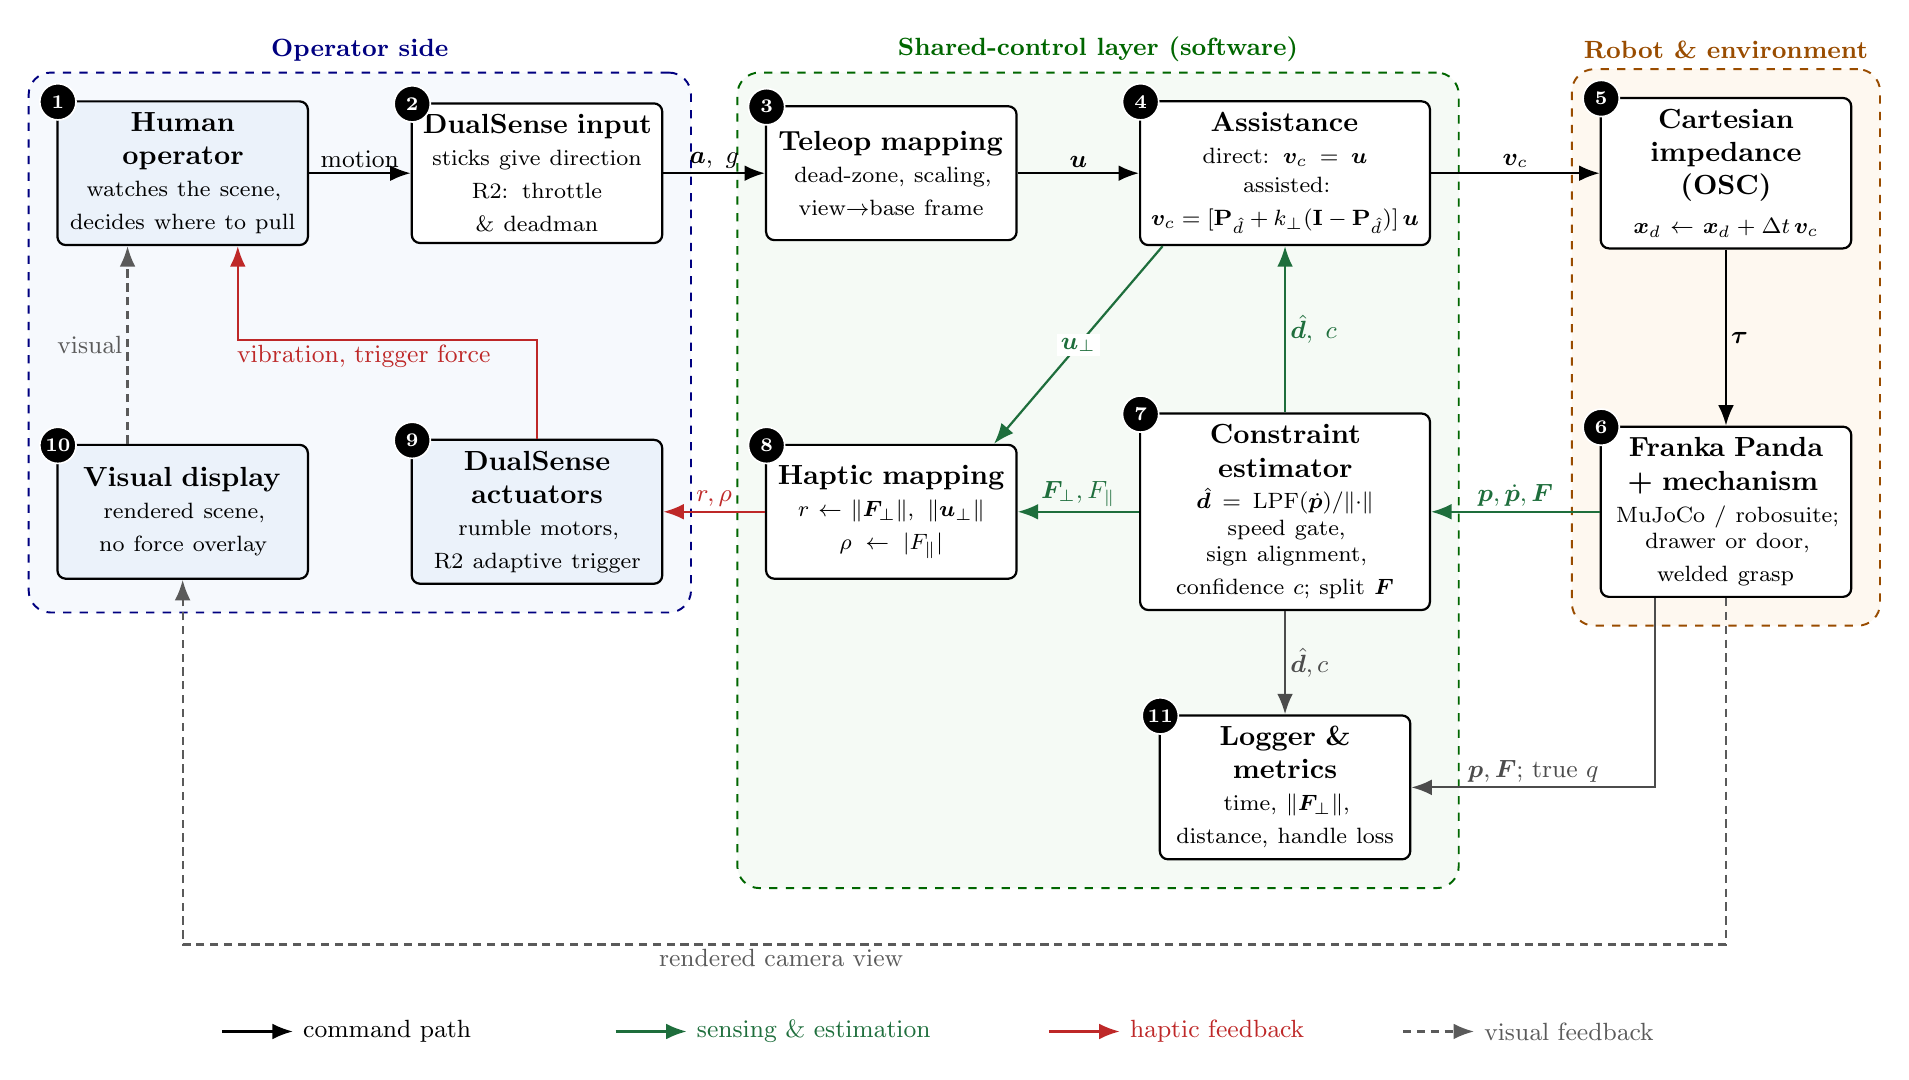
\begin{tikzpicture}[
  font=\normalsize,
  blk/.style={draw, thick, rounded corners=3pt, fill=white, align=center,
              text width=2.9cm, minimum height=1.7cm, inner sep=4pt},
  wide/.style={blk, text width=3.4cm},
  sig/.style={-{Latex[length=2.6mm,width=2mm]}, thick},
  hap/.style={sig, hapcol},
  vis/.style={sig, viscol, densely dashed},
  est/.style={sig, estcol},
  lab/.style={font=\small, inner sep=1.5pt, align=center},
  num/.style={circle, draw=white, line width=0.6pt, fill=black, text=white,
              font=\scriptsize\bfseries, inner sep=0.5pt, minimum size=4.6mm},
  grp/.style={draw, rounded corners=8pt, dashed, line width=0.7pt, inner sep=10pt},
]

% ----- row A: forward path
\node[blk, fill=opcol!70] (human) at (0,0)
     {\textbf{Human operator}\\[2pt]\footnotesize watches the scene,\\ decides where to pull};
\node[blk] (dsin) at (4.5,0)
     {\textbf{DualSense input}\\[2pt]\footnotesize sticks give direction\\ R2: throttle \& deadman};
\node[blk] (map) at (9.0,0)
     {\textbf{Teleop mapping}\\[2pt]\footnotesize dead-zone, scaling,\\ view$\to$base frame};
\node[wide] (assist) at (14.0,0)
     {\textbf{Assistance}\\[2pt]\footnotesize direct: $\vcmd=\vuser$\\[1pt]
      assisted:\\ $\vcmd=[\Pd+k_\perp(\I-\Pd)]\,\vuser$};
\node[blk] (ctrl) at (19.6,0)
     {\textbf{Cartesian\\ impedance (OSC)}\\[2pt]\footnotesize $\vect x_d \leftarrow \vect x_d+\Delta t\,\vcmd$};

% ----- row B: feedback path
\node[blk, fill=opcol!70] (disp) at (0,-4.3)
     {\textbf{Visual display}\\[2pt]\footnotesize rendered scene,\\ no force overlay};
\node[blk, fill=opcol!70] (dsout) at (4.5,-4.3)
     {\textbf{DualSense actuators}\\[2pt]\footnotesize rumble motors,\\ R2 adaptive trigger};
\node[blk] (hap) at (9.0,-4.3)
     {\textbf{Haptic mapping}\\[2pt]\footnotesize $r \leftarrow \lVert\Fperp\rVert,\ \lVert\vuser_\perp\rVert$\\
      $\rho \leftarrow |\Fpar|$};
\node[wide, minimum height=2.0cm] (est) at (14.0,-4.3)
     {\textbf{Constraint estimator}\\[2pt]\footnotesize $\hat{\vect d}=\mathrm{LPF}(\dot{\vect p})/\lVert\cdot\rVert$\\
      speed gate, sign alignment,\\ confidence $c$;\ split $\Fext$};
\node[blk, minimum height=2.0cm] (sim) at (19.6,-4.3)
     {\textbf{Franka Panda\\ + mechanism}\\[2pt]\footnotesize MuJoCo / robosuite;\\ drawer or door,\\ welded grasp};

% ----- row C
\node[blk] (log) at (14.0,-7.8)
     {\textbf{Logger \& metrics}\\[2pt]\footnotesize time, $\lVert\Fperp\rVert$,\\ distance, handle loss};

% ----- block numbers (on the upper-left corner)
\foreach \n/\k in {human/1,dsin/2,map/3,assist/4,ctrl/5,sim/6,est/7,hap/8,dsout/9,disp/10,log/11}
  \node[num] at ($(\n.north west)+(0.02,-0.02)$) {\k};

% ----- forward (command) path
\draw[sig] (human) -- node[lab, above] {motion} (dsin);
\draw[sig] (dsin) -- node[lab, above] {$\vect a,\ g$} (map);
\draw[sig] (map) -- node[lab, above] {$\vuser$} (assist);
\draw[sig] (assist) -- node[lab, above] {$\vcmd$} (ctrl);
\draw[sig] (ctrl) -- node[lab, right] {$\bm\tau$} (sim);

% ----- estimator and sensing path
\draw[est] (sim) -- node[lab, above] {$\vect p,\dot{\vect p},\Fext$} (est);
\draw[est] (est) -- node[lab, right] {$\hat{\vect d},\ c$} (assist);
\draw[est] (est) -- node[lab, above] {$\Fperp,\Fpar$} (hap);
\draw[est] ($(assist.south west)+(0.3,0)$) -- node[lab, fill=white, pos=0.5] {$\vuser_\perp$} ($(hap.north east)+(-0.3,0)$);

% ----- haptic feedback to the operator
\draw[hap] (hap) -- node[lab, above] {$r,\rho$} (dsout);
\draw[hap] (dsout.north) -- ++(0,1.25) coordinate (hk) -| ($(human.south)+(0.7,0)$);
\node[lab, text=hapcol, below] at ($(hk)+(-2.2,0)$) {vibration, trigger force};

% ----- visual feedback
\draw[vis] (sim.south) -- ++(0,-4.4) coordinate (vk) -| (disp.south);
\node[lab, text=viscol, below] at ($(vk)+(-12.0,0)$) {rendered camera view};
\draw[vis] ($(disp.north)+(-0.7,0)$) -- node[lab, text=viscol, left] {visual} ($(human.south)+(-0.7,0)$);

% ----- logging and ground truth
\draw[sig, black!70] ($(sim.south)+(-0.9,0)$) |- node[lab, pos=0.75, above] {$\vect p,\Fext$; true $q$} (log.east);
\draw[sig, black!70] (est) -- node[lab, right] {$\hat{\vect d},c$} (log);

% ----- groups
\begin{scope}[on background layer]
  \node[grp, draw=blue!50!black, fill=opcol!30, fit=(human)(dsin)(dsout)(disp)] (G1) {};
  \node[grp, draw=green!40!black, fill=sccol!45, fit=(map)(assist)(est)(hap)(log)] (G2) {};
  \node[grp, draw=orange!60!black, fill=robcol!50, fit=(ctrl)(sim)] (G3) {};
\end{scope}
\node[font=\small\bfseries, text=blue!50!black, anchor=south] at (G1.north) {Operator side};
\node[font=\small\bfseries, text=green!40!black, anchor=south] at (G2.north) {Shared-control layer (software)};
\node[font=\small\bfseries, text=orange!60!black, anchor=south] at (G3.north) {Robot \& environment};

% ----- legend (single row under the diagram)
\begin{scope}[shift={(0.5,-10.9)}, font=\small]
  \draw[sig] (0,0) -- (0.9,0) node[right] {command path};
  \draw[est] (5,0) -- (5.9,0) node[right] {sensing \& estimation};
  \draw[hap] (10.5,0) -- (11.4,0) node[right] {haptic feedback};
  \draw[vis] (15,0) -- (15.9,0) node[right] {visual feedback};
\end{scope}
\end{tikzpicture}%
}
\caption{Annotated block diagram of the proposed shared-control architecture. Numbered blocks are described in \cref{tab:blocks}. Under \emph{direct} control block~4 passes the operator command through unchanged; under \emph{assisted} control it projects the command onto the estimated tangent $\hat{\vect d}$ supplied by block~7. The operator receives two feedback channels: the rendered scene (dashed grey) and the DualSense haptics (red). The ground-truth joint coordinate $q$ of the mechanism reaches only the logger and is never available to the controller or the estimator.}
\label{fig:block}
\end{figure}
\end{landscape}
}


The proposed control architecture is shown in \cref{fig:block}, with each numbered block described in \cref{tab:blocks}. Its components fall into three groups. On the operator side, the DualSense controller serves both as the input device and as the haptic display. The shared-control layer contains the teleoperation mapping, the assistance block, the constraint estimator, the haptic mapping and the logger. The robot and environment group comprises a Cartesian impedance controller and a simulated Franka Panda holding the handle of a drawer or door. The forward path carries the operator's intent to the robot, and two feedback paths return information to the operator, one visual through the rendered scene and one haptic through the controller. A third, internal path carries measured motion and force from the robot to the estimator, and it is this path that makes the system a shared controller rather than a filtered teleoperator.

Every signal crossing the boundary of the shared-control layer is a Cartesian vector or a scalar, so the layer is independent of the simulator. The intended platform is robosuite \cite{zhu2020robosuite} running on MuJoCo \cite{todorov2012mujoco}, which provides a Panda model with operational-space control, a hinged-door task and DualSense input; haptic output is added through \texttt{pydualsense} \cite{pydualsense}, and a prismatic drawer with configurable axis orientation is added as a custom model. The same layer could equally drive a Gazebo model through ROS~2 or, eventually, physical hardware.




\subsection{Problem Setting}
\label{sec:setting}

Let $\vect p\in\mathbb R^3$ denote the position of the grasp point in the robot base frame and $\dot{\vect p}$ its velocity. The mechanism permits motion along a path $\vect p(q)$ parameterised by its joint coordinate $q$. For a drawer the path is a straight line, $\vect p(q)=\vect p_0+q\,\vect d^\star$, with constant unit axis $\vect d^\star$; for a door it is a circular arc of radius $\varrho$ about the hinge, and the unit tangent $\vect d^\star(q)$ rotates with the opening angle. In either case the admissible velocities form the one-dimensional subspace spanned by $\vect d^\star$, which is unknown to the controller; both geometries are sketched in \cref{fig:geometry}. Given the external force $\Fext$ measured at the wrist, the along-path and off-axis components with respect to the current estimate are
\begin{equation}
  \Fpar = \hat{\vect d}^{\top}\Fext, \qquad
  \Fperp = \bigl(\I-\hat{\vect d}\hat{\vect d}^{\top}\bigr)\Fext,
  \label{eq:forcesplit}
\end{equation}
and the rejected part of the operator command is $\vuser_\perp=(\I-\hat{\vect d}\hat{\vect d}^{\top})\vuser$. For evaluation these quantities are recomputed with the ground-truth tangent $\vect d^\star$, so that a biased estimate cannot conceal off-axis force. Because the grasp is welded in simulation, handle loss is registered whenever $\lVert\Fperp\rVert$ exceeds a slip threshold that a real parallel gripper could not sustain.



\subsection{Constraint Estimation}
\label{sec:estimator}



The estimator follows \cite{lutscher2010control} with three practical additions: a speed gate, sign alignment and a confidence measure. The measured velocity is first low-pass filtered, $\bar{\vect v}_k = (1-\beta)\,\bar{\vect v}_{k-1} + \beta\,\dot{\vect p}_k$ with $0<\beta\le 1$. Whenever $\lVert\bar{\vect v}_k\rVert$ exceeds a threshold $v_{\min}$, the unit vector $\vect m_k=\bar{\vect v}_k/\lVert\bar{\vect v}_k\rVert$ is accepted as a direction sample, flipped if $\vect m_k^{\top}\hat{\vect d}_{k-1}<0$ since $\vect d$ and $-\vect d$ span the same subspace. The last $N$ samples, held in a window $\mathcal W_k$, give
\begin{equation}
  \hat{\vect d}_k = \frac{\sum_{\vect m\in\mathcal W_k}\vect m}{\bigl\lVert\sum_{\vect m\in\mathcal W_k}\vect m\bigr\rVert},
  \qquad
  c_k = \frac{1}{N}\Bigl\lVert\sum_{\vect m\in\mathcal W_k}\vect m\Bigr\rVert \in[0,1].
  \label{eq:estimator}
\end{equation}
The confidence $c_k$, the mean resultant length of the samples, approaches one when recent motion has been consistently along one line and falls when the samples disagree, as they do at start-up. Below the speed gate the previous estimate is held.

% ---------------------- block description table --------------------
\begin{table}[tb]
\centering
\caption{Description of the numbered blocks and signals in \cref{fig:block}.}
\label{tab:blocks}
\footnotesize
\renewcommand{\arraystretch}{1.18}
\begin{tabularx}{\textwidth}{@{}c>{\raggedright\arraybackslash}p{2.7cm}>{\raggedright\arraybackslash}X>{\raggedright\arraybackslash}p{3.2cm}@{}}
\toprule
\textbf{\#} & \textbf{Block} & \textbf{Function} & \textbf{Outputs} \\
\midrule
1 & Human operator & Chooses the target, judges progress from the rendered scene and reacts to haptic cues. & Thumb and finger motion \\
2 & DualSense input & Left stick sets planar direction and right stick vertical direction; R2 depression $g\in[0,1]$ scales speed and acts as a deadman. & Stick axes $\vect a$, throttle $g$ \\
3 & Teleop mapping & Dead-zone, speed limit $v_{\max}$ and rotation from the viewing frame to the robot base frame. & $\vuser = g\,v_{\max}\,\mathbf{R}\,\phi(\vect a)$ \\
4 & Assistance & Passes $\vuser$ unchanged (direct) or applies the confidence-weighted guidance fixture of \eqref{eq:assist} (assisted). & $\vcmd$ \\
5 & Cartesian impedance / OSC & Integrates $\vcmd$ into a desired pose and tracks it compliantly, so that the mechanism can deflect the end-effector. & Joint torques $\bm\tau$ \\
6 & Franka Panda + mechanism & Simulated arm, welded grasp and prismatic drawer or revolute door with friction and damping; axis orientation randomised per trial. & $\vect p,\ \dot{\vect p},\ \Fext$; ground truth $q$ \\
7 & Constraint estimator & Filtered, gated and sign-aligned tangent estimate (\cref{alg:loop}); splits the wrench into along-path and off-axis parts. & $\hat{\vect d}$, confidence $c$, $\Fpar$, $\Fperp$ \\
8 & Haptic mapping & Maps off-axis force and rejected command to rumble intensity $r$, and along-path force to trigger resistance $\rho$. & $r,\ \rho\in[0,1]$ \\
9 & DualSense actuators & Rumble motors and R2 adaptive trigger. & Vibration, trigger force \\
10 & Visual display & Rendered view of robot and mechanism, identical in both modes. & Visual feedback \\
11 & Logger \& metrics & Records all signals; computes opening time, off-axis force, handle-loss events and opening distance. & Time series, metrics \\
\bottomrule
\end{tabularx}
\end{table}

\begin{figure}[t]
\centering
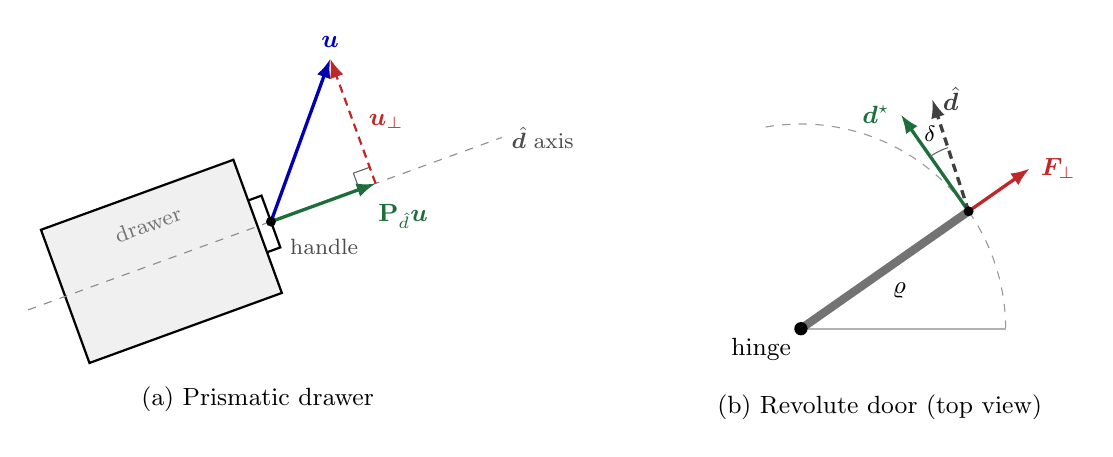
\begin{tikzpicture}[
  >={Latex[length=2.4mm]}, font=\small,
  vec/.style={->, very thick},
]
% ---------------- (a) drawer -----------------
\begin{scope}
  \begin{scope}[rotate=20]
    \fill[black!6] (-2.6,-0.9) rectangle (0,0.9);
    \draw[thick] (-2.6,-0.9) rectangle (0,0.9);
    \draw[black!45, dashed] (-3.1,0) -- (3.3,0) node[right, black!70, font=\footnotesize] {$\hat{\vect d}$ axis};
    \node[black!55, font=\footnotesize, rotate=20] at (-1.3,0.5) {drawer};
    \draw[thick] (0,-0.35) -- (0.18,-0.35) -- (0.18,0.35) -- (0,0.35);
  \end{scope}
  \coordinate (H) at (0.17,0.06);
  \coordinate (U) at ($(H)+(70:2.2)$);
  \coordinate (Pu) at ($(H)+(20:{2.2*cos(50)})$);
  \pic[draw, black!60, angle radius=2.2mm] {right angle = H--Pu--U};
  \draw[vec, blue!70!black] (H) -- (U) node[above] {$\vuser$};
  \draw[vec, estcol] (H) -- (Pu);
  \node[estcol, font=\small] at ($(Pu)+(0.35,-0.42)$) {$\Pd\vuser$};
  \draw[densely dashed, hapcol, thick, ->] (Pu) -- (U) node[midway, right=2pt] {$\vuser_\perp$};
  \fill (H) circle (1.8pt);
  \node[font=\footnotesize, black!70, anchor=north west] at ($(H)+(0.12,-0.1)$) {handle};
  \node at (0,-2.2) {(a) Prismatic drawer};
\end{scope}

% ---------------- (b) door -----------------
\begin{scope}[shift={(6.9,-1.3)}]
  \draw[black!40, dashed] (0:2.6) arc (0:100:2.6);
  \draw[black!30, thick] (0,0) -- (0:2.6);
  \draw[line width=3pt, black!55] (0,0) -- (35:2.6);
  \fill (0,0) circle (2.4pt) node[below left] {hinge};
  \coordinate (H2) at (35:2.6);
  \draw[vec, estcol] (H2) -- ++(125:1.5) node[left] {$\vect d^\star$};
  \draw[vec, densely dashed, black!75] (H2) -- ++(108:1.5) node[right] {$\hat{\vect d}$};
  \draw[black!60] ($(H2)+(108:0.85)$) arc (108:125:0.85);
  \node[font=\footnotesize] at ($(H2)+(116.5:1.1)$) {$\delta$};
  \draw[vec, hapcol] (H2) -- ++(35:0.95) node[right] {$\Fperp$};
  \fill (H2) circle (1.8pt);
  \node[font=\small] at ($(35:1.3)+(-55:0.32)$) {$\varrho$};
  \node at (1.0,-1.0) {(b) Revolute door (top view)};
\end{scope}\end{tikzpicture}
\caption{Geometry of the assistance. (a)~On a drawer, the operator's command $\vuser$ is split into the part along the estimated axis, which is executed, and the rejected part $\vuser_\perp$, which is removed under assisted control and reported by vibration. (b)~On a door, the true tangent $\vect d^\star$ rotates as the door opens; the filtered estimate $\hat{\vect d}$ trails it by a small angle $\delta$ (exaggerated here for clarity), so a small radial force $\Fperp$ remains and is absorbed by the controller's compliance.}
\label{fig:geometry}
\end{figure}


The estimator remains valid when assistance is active, for a reason rooted in the physics of compliant contact. The mechanism forces the end-effector onto its path, so the measured velocity points along $\vect d^\star$ whatever the commanded direction, provided the command has a non-zero component along $\vect d^\star$. An erroneous estimate therefore still produces motion in the correct direction, and the estimate corrects itself. Only an estimate exactly perpendicular to $\vect d^\star$ would stall a hard fixture, a case avoided by the soft fixture of \cref{sec:assist}. On a door, where the tangent rotates at $\omega=\lVert\dot{\vect p}\rVert/\varrho$, a filter with effective time constant $T_f$ causes the estimate to lag by approximately
\begin{equation}
  \delta \approx \omega\,T_f = \frac{\lVert\dot{\vect p}\rVert\,T_f}{\varrho}.
  \label{eq:lag}
\end{equation}
A handle speed of $0.1$~m/s, a radius of $0.5$~m and $T_f=0.2$~s give $\delta\approx0.04$~rad, so roughly 4\% of the commanded speed leaks into the radial direction, an amount a compliant controller absorbs easily. The same relation exposes the trade-off in choosing $T_f$: heavier filtering suppresses noise but increases lag, and does so more severely on mechanisms of small radius.

\begin{algorithm}[tb]
\caption{One cycle of the shared-control loop (assisted mode).}
\label{alg:loop}
\begin{algorithmic}[1]
\Require window size $N$, filter gain $\beta$, speed gate $v_{\min}$, gains $k_{\min},c_0,c_1$
\State $(\vect a, g) \gets$ \Call{ReadDualSense}{}
\State $\vuser \gets g\,v_{\max}\,\mathbf R\,\phi(\vect a)$ \Comment{dead-zone, scaling, frame}
\State $(\vect p,\dot{\vect p},\Fext) \gets$ \Call{ReadRobotState}{}
\State $\bar{\vect v} \gets (1-\beta)\bar{\vect v} + \beta\dot{\vect p}$
\If{$\lVert\bar{\vect v}\rVert > v_{\min}$}
  \State $\vect m \gets \bar{\vect v}/\lVert\bar{\vect v}\rVert$
  \If{$\vect m^{\top}\hat{\vect d} < 0$} \State $\vect m \gets -\vect m$ \EndIf
  \State push $\vect m$ into $\mathcal W$ (drop oldest if $|\mathcal W|>N$)
  \State $\hat{\vect d} \gets \sum\mathcal W/\lVert\sum\mathcal W\rVert$;\quad $c \gets \lVert\sum\mathcal W\rVert/N$
\EndIf
\State $\Pd \gets \hat{\vect d}\hat{\vect d}^{\top}$;\quad $k_\perp \gets k_\perp(c)$ from \eqref{eq:assist}
\State $\vcmd \gets [\Pd + k_\perp(\I-\Pd)]\vuser$ \Comment{$\vcmd\gets\vuser$ under direct control}
\State $\Fpar \gets \hat{\vect d}^{\top}\Fext$;\quad $\Fperp \gets (\I-\Pd)\Fext$;\quad $\vuser_\perp \gets (\I-\Pd)\vuser$
\State send $r$ and $\rho$ from \eqref{eq:haptic} to the DualSense
\State $\vect x_d \gets \vect x_d + \Delta t\,\vcmd$; \Call{SendToController}{$\vect x_d$}
\State \Call{Log}{all signals, ground-truth $q$}
\end{algorithmic}
\end{algorithm}

\subsection{Assistance and Low-Level Control}
\label{sec:assist}

Under direct control the command passes through unchanged, $\vcmd=\vuser$. Under assisted control a guidance virtual fixture \cite{marayong2003spatial} is built from the current estimate,
\begin{equation}
  \vcmd = \bigl[\,\Pd + k_\perp(c_k)\,(\I-\Pd)\,\bigr]\,\vuser,
  \qquad
  k_\perp(c) = 1 - (1-k_{\min})\,\sat_{[0,1]}\!\left(\frac{c-c_0}{c_1-c_0}\right),
  \label{eq:assist}
\end{equation}
with $\Pd=\hat{\vect d}_k\hat{\vect d}_k^{\top}$. While confidence is low ($c\le c_0$) the operator retains full authority and the system behaves exactly as under direct control; this is the start-up phase in which the operator's own pulling reveals the mechanism. As the samples align, $k_\perp$ falls towards a small value $k_{\min}$, for instance $0.05$, and the fixture becomes effectively hard. Keeping $k_{\min}>0$ preserves a little operator authority in every direction, which prevents the stall described above and allows recovery from a badly wrong estimate. This confidence-dependent gain is a simple realisation of the adaptive autonomy discussed by Li et al.\ \cite{li2023classification}. The end-effector orientation is held fixed for the drawer; for the door, the rotational stiffness about the vertical axis is kept low so that the wrist can turn with the door.

The commanded velocity is integrated into a desired position, $\vect x_{d,k+1}=\vect x_{d,k}+\Delta t\,\vcmd$, which is tracked by operational-space control \cite{khatib1987unified},
\begin{equation}
  \bm\tau = \mathbf J^{\top}\bm\Lambda\bigl[\mathbf K_p(\vect x_d-\vect x)-\mathbf K_d\dot{\vect x}\bigr] + \bm\tau_g + \bm\tau_{\mathrm{null}},
  \label{eq:osc}
\end{equation}
where $\bm\Lambda$ is the operational-space inertia, $\mathbf K_p$ and $\mathbf K_d$ are stiffness and damping gains, $\bm\tau_g$ compensates gravity and $\bm\tau_{\mathrm{null}}$ regulates the redundant degree of freedom. This impedance law \cite{hogan1985impedance} also explains where off-axis force originates. With the handle constrained, the tracking error $\vect x_d-\vect x$ can grow only in the blocked directions, and the force exerted on the mechanism is approximately $\mathbf K_p$ times that error. Under direct control, any lateral component of $\vuser$ integrates into a growing lateral error and hence a growing $\Fperp$; under assisted control that component is removed at its source. A moderate translational stiffness ensures that residual errors, such as the filter lag in \eqref{eq:lag}, generate only small forces.

\subsection{Haptic Feedback}
\label{sec:haptics}

The two haptic channels carry two quantities with distinct meanings, so that the operator does not have to disentangle them. Vibration indicates that the operator is pushing against the mechanism, and combines the measured off-axis force with the rejected part of the command; trigger resistance indicates that the mechanism itself is hard to open:
\begin{equation}
  r = \sat_{[0,1]}\!\left(\frac{\lVert\Fperp\rVert-F_0}{F_1-F_0} + \kappa_u\frac{\lVert\vuser_\perp\rVert}{v_{\max}}\right),
  \qquad
  \rho = \sat_{[0,1]}\!\left(\frac{|\Fpar|-F_{\parallel,0}}{F_{\parallel,1}-F_{\parallel,0}}\right).
  \label{eq:haptic}
\end{equation}
The force term in $r$ responds to physical resistance from the mechanism, whereas the command term responds to what the fixture discards silently, which matters under assistance because off-axis force may stay small even when the operator steers poorly. The dead-zones $F_0$ and $F_{\parallel,0}$ suppress cues caused by sensor noise and gripper inertia. Since R2 also serves as the throttle, the operator feels opening resistance in the same finger that requests motion. In line with the findings of Boulay et al.\ \cite{boulay2026selecting}, the thresholds and the weight $\kappa_u$ are to be set from force ranges observed in pilot trials, and the same haptic laws apply in both modes. One complete cycle of the resulting control loop is summarised in \cref{alg:loop}.



% ==================================================================
\section{Conclusion}
\label{sec:conclusion}

This paper has reviewed the work most relevant to teleoperated opening of an unfamiliar drawer or door and has proposed an architecture for studying it. The primary paper, Lutscher et al.\ \cite{lutscher2010control}, offers a compact and well-founded means of estimating the permitted motion of an unknown mechanism from the robot's own motion. Recent research on articulation estimation confirms that interaction data are the most dependable source of this information once contact is established, while research on shared control and haptics supplies both the form of the assistance and the means of informing the operator. The resulting design projects the operator's DualSense command onto the online-estimated tangent, introduces assistance gradually as the estimate gains confidence, and reports off-axis loading through vibration and opening resistance through the adaptive trigger. Because direct and assisted control share identical feedback, the architecture allows the effect of assistance on opening time, off-axis force, handle loss and opening distance to be isolated in a controlled comparison.

% ==================================================================
\printbibliography[heading=bibintoc,title={References}]

\end{document}
